\subsection{Получение вольт-амперной характеристики на экране осциллографа (динамический метод)}

При максимальном ускоряющем напряжении измерим на экране расстояние между
максимумами и между минимумами осциллограммы. Измерения проведём при трёх
значениях задерживающего напряжения: $4$, $6$ и $8$ В. Результаты измерений занесём в
таблицу \ref{tab::dyn}.

\begin{table}[h!]
  \centering
  \captionsetup{justification=centering}
  \caption{Измерения максимумов и минимумов напряжений ВАХ на осциллографе}
  \begin{tabular}{|c|c|c|c|c|c|}
    \hline
    $V_2$, В & $V_{max_1}$, В & $V_{max_2}$, В & $V_{min_1}$, В & $V_{min_2}$, В & $\sigma_V$, В \\
    \hline
    4 & 0 & 13 & 2 & 19 & 1  \\
    \hline
    6 & -4 & 10 & 0 & 17.5 & 1  \\
    \hline
    8 & -4 & 10 & 0 & 18 & 1  \\
    \hline
  \end{tabular}

  \begin{tabular}{|c|c|c|c|c|}
    \hline
    $V_2$, В  & $\Delta V_{max}$, В & $\sigma_{\Delta V_{max}}$, В& $\Delta V_{min}$, В &$ \sigma_{\Delta V_{min}}$, В \\
    \hline
    4 &  13.0 & 1.4 & 17.0 & 1.4   \\
    \hline
    6 &  14.0 & 1.4 & 17.5 & 1.4   \\
    \hline
    8 &  14.0 & 1.4 & 18.0 & 1.4   \\
    \hline
  \end{tabular}

  \label{tab::dyn}
\end{table}

Исходя из полученных данных, определим значение энергии первого возбуждённого
состояния атома гелия. Для этого сначала усредним полученные значения разности минимумов и максимумов:
\begin{align*}
  \mean{\Delta V_{max}} = 13 \pm 2 \: В && \mean{\Delta V_{min }} = 18 \pm 2 \: В
\end{align*}
Усредняя их, получаем в итоге:
\begin{equation*}
  \mean{\Delta V_{дин}} = 16 \pm 4 \: В
\end{equation*}
Таким образом, для значения энергии первого возбуждённого состояния атома гелия
по результатам эксперимента имеем:

\begin{equation}
  \Delta E_{дин} = 16 \pm 4 \: эВ
\end{equation}

\subsection{Получение вольт-амперной характеристики в статическом режиме измерений}

Снимем зависимость коллекторного тока от анодного напряжения $I_k = f(V_a)$ для
значений задерживающего напряжения $4$, $6$ и $8$ В. По измеренным данным
построим график \ref{img::VAC}.


\begin{figure}[h!]
  \centering
  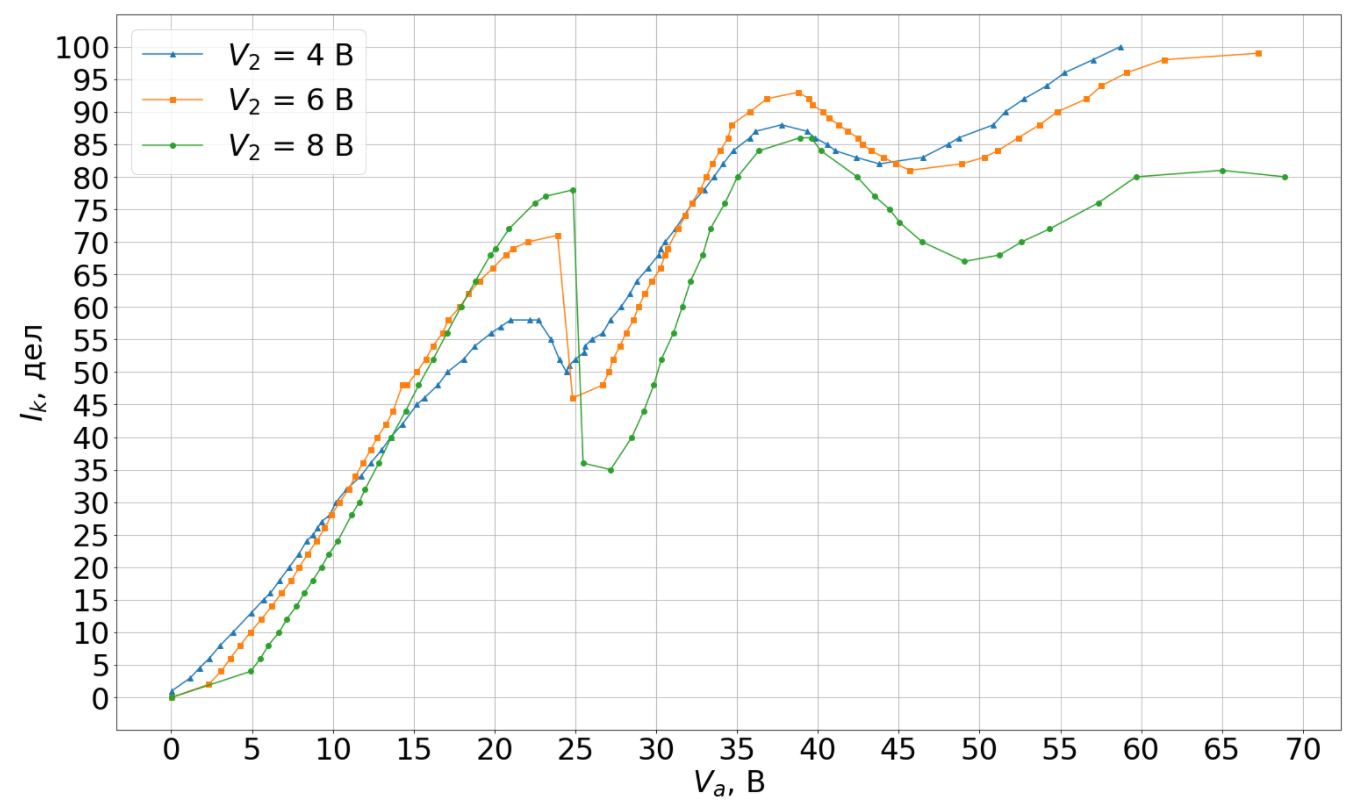
\includegraphics[width=1\linewidth]{VAC.png}
  \captionsetup{justification=centering}
  \caption{ВАХ трёхэлектродной вакуумной лампы при различных значениях запирающего напряжения}
  \label{img::VAC}
\end{figure}

По графику определим точки максимумов и минимумов, результаты занесём в таблицу \ref{tab::stat}.

\begin{table}
  \centering
  \captionsetup{justification=centering}
  \caption{Измерения максимумов и минимумов напряжений ВАХ по графику}
  \begin{tabular}{|c|c|c|c|c|c|}
    \hline
    $V_2$, В & $V_{max_1}$, В & $V_{max_2}$, В & $V_{min_1}$, В & $V_{min_2}$, В & $\sigma_V$, В \\
    \hline
    4 & 23 & 38 & 25 & 45 & 1  \\
    \hline
    6 & 24 & 39 & 25 & 48 & 1  \\
    \hline
    8 & 25 & 40 & 28 & 50 & 1  \\
    \hline
  \end{tabular}

  \begin{tabular}{|c|c|c|c|c|}
    \hline
    $V_2$, В  & $\Delta V_{max}$, В & $\sigma_{\Delta V_{max}}$, В& $\Delta V_{min}$, В &$ \sigma_{\Delta V_{min}}$, В \\
    \hline
    4 &  15 & 1.4 & 20 & 1.4   \\
    \hline
    6 &  15 & 1.4 & 23 & 1.4   \\
    \hline
    8 &  15 & 1.4 & 22 & 1.4   \\
    \hline
  \end{tabular}

  \label{tab::stat}
\end{table}

Исходя из полученных данных, определим значение энергии первого возбуждённого
состояния атома гелия. Для этого сначала усредним полученные значения разности минимумов и максимумов:
\begin{align*}
  \mean{\Delta V_{max}} = 15 \pm 2 \: В && \mean{\Delta V_{min }} = 22 \pm 2 \: В
\end{align*}
Усредняя их, получаем в итоге:
\begin{equation*}
  \mean{\Delta V_{стат}} = 18 \pm 4 \: В
\end{equation*}
Таким образом, для значения энергии первого возбуждённого состояния атома гелия
по результатам эксперимента имеем:

\begin{equation}
  \Delta E_{стат} = 18 \pm 4 \: эВ
\end{equation}